\documentclass{standalone}

\usepackage{tikz}

\begin{document}

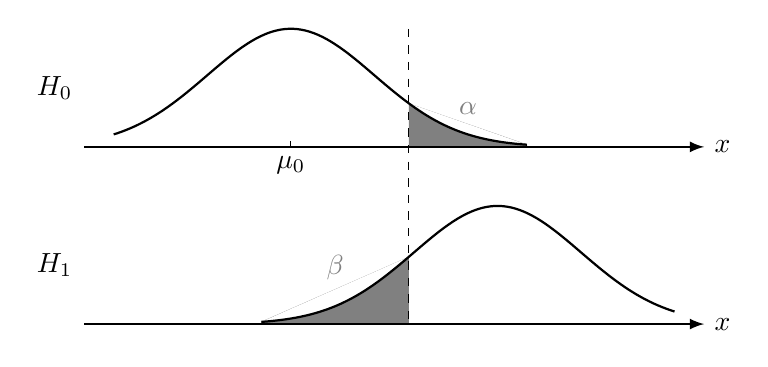
\begin{tikzpicture}[>=latex, xscale=1.5, yscale=1.5]
    \node at(-2, .5){$H_0$};
    \node at(-2, -1){$H_1$};
    \fill[gray](1, 0)--(1, .368)--(2, .02)node[midway, above]{$\alpha$}--(2, 0);
    \fill[white, domain=1:2]plot(\x,{exp(-\x*\x)});
    \fill[gray, shift={(1.75, -1.5)}](-.75, 0)--(-.75, .57)--(-2, .02)node[midway, above]{$\beta$}--(-2, 0);
    \fill[white, domain=-2:-.75, shift={(1.75, -1.5)}]plot(\x,{exp(-\x*\x)});
    \draw[dashed](1, 1)--(1, -1.5);
    \draw[thick, -latex](-1.75, 0)--(3.5, 0)node[right]{$x$};
    \draw(0, .05)--(0, 0)node[below]{$\mu_0$};
    \draw[thick, domain=-1.5:2, samples=100]plot(\x,{exp(-\x*\x)});
    \draw[thick, -latex](-1.75, -1.5)--(3.5, -1.5)node[right]{$x$};
    \draw[thick, domain=-2:1.5, samples=100, shift={(1.75, -1.5)}]plot(\x,{exp(-\x*\x)});
\end{tikzpicture}

\end{document}